\documentclass{beamer}
\usepackage{tikz}
\usetikzlibrary{shapes.geometric, arrows.meta, positioning}

% Beamer theme
\usetheme{JuanLesPins}

% Title page details
\title{Iris Detection using Mediapipe and Python}
\author{Rajesh G.D.}
\date{\today}

\begin{document}
	
	% Title Slide
	\begin{frame}
		\titlepage
	\end{frame}
	
	% Slide 1: What is Iris Detection?
	\begin{frame}{What is Iris Detection?}
		\centering
		\includegraphics[width=0.5\linewidth]{iris_image.jpg}
		\begin{itemize}
			\item \textbf{Iris Detection} is a computer vision task aimed at detecting and tracking the iris of the human eye in real-time.
			\item The iris is the colored part of the eye surrounding the pupil. Its shape and position are crucial in biometric identification, gaze tracking, and medical diagnostics.
			\item Iris detection can be used in:
			\begin{itemize}
				\item Eye-tracking systems
				\item Augmented reality (AR) applications
				\item User authentication (biometrics)
			\end{itemize}
			\item Challenges include accurately tracking iris movements under various lighting and head pose conditions.
		\end{itemize}
	\end{frame}
	
	% Slide 2: How does Mediapipe Work for Iris Detection?
	\begin{frame}{How does Mediapipe Work for Iris Detection?}
		\begin{itemize}
			\item \textbf{Mediapipe} is a framework by Google for building multimodal, cross-platform machine learning pipelines.
			\item For iris detection, Mediapipe's \textbf{Face Mesh} uses 468 3D landmarks to map facial features, including eyes.
			\item Key Features of Mediapipe for Iris Detection:
			\begin{itemize}
				\item Accurate real-time face and eye landmark detection.
				\item Refinement of eye landmarks with an additional 5-point iris model.
				\item Works on multiple platforms, including web, mobile, and desktop.
			\end{itemize}
			\item Mediapipe is known for its efficiency and high performance with minimal computational resources.
		\end{itemize}
	\end{frame}
	% A slide in between for mediapipe landmarks
	\begin{frame}
		\includegraphics[width=0.9\linewidth]{$HOME/Pictures/mediapipe_landmarks.jpg}
	\end{frame}
	
	% landmarks in documentation
	\begin{frame}
		FACEMESH_LEFT_EYE = frozenset([(263, 249), (249, 390), (390, 373), (373, 374),
		(374, 380), (380, 381), (381, 382), (382, 362),
		(263, 466), (466, 388), (388, 387), (387, 386),
		(386, 385), (385, 384), (384, 398), (398, 362)])
		
		FACEMESH_LEFT_IRIS = frozenset([(474, 475), (475, 476), (476, 477),
		(477, 474)])
		
		FACEMESH_LEFT_EYEBROW = frozenset([(276, 283), (283, 282), (282, 295),
		(295, 285), (300, 293), (293, 334),
		(334, 296), (296, 336)])
		
		FACEMESH_RIGHT_EYE = frozenset([(33, 7), (7, 163), (163, 144), (144, 145),
		(145, 153), (153, 154), (154, 155), (155, 133),
		(33, 246), (246, 161), (161, 160), (160, 159),
		(159, 158), (158, 157), (157, 173), (173, 133)])
		
		FACEMESH_RIGHT_EYEBROW = frozenset([(46, 53), (53, 52), (52, 65), (65, 55),
		(70, 63), (63, 105), (105, 66), (66, 107)])
		
		FACEMESH_RIGHT_IRIS = frozenset([(469, 470), (470, 471), (471, 472),
		(472, 469)])
	\end{frame}
	% Slide 3: Step 1 - Import Libraries
	\begin{frame}[fragile]{Step 1: Import Necessary Libraries}
		\tiny
		\begin{verbatim}
			import cv2
			import mediapipe as mp
			import numpy as np
			import csv
			import os
			import time
		\end{verbatim}
		\begin{itemize}
			\item This step includes importing the necessary libraries:
			\begin{itemize}
				\item \texttt{cv2}: For handling video input and image processing.
				\item \texttt{mediapipe}: For face landmark detection.
				\item \texttt{numpy}: For numerical operations and calculations.
				\item \texttt{csv}: For handling CSV file operations.
				\item \texttt{os}: For file and directory operations.
				\item \texttt{time}: For handling timing operations.
			\end{itemize}
		\end{itemize}
	\end{frame}
	
	% Slide 4: Step 2 - Remove Existing CSV File
	\begin{frame}[fragile]{Step 2: Remove Existing CSV File}
		\tiny
		\begin{verbatim}
			csv_file = 'iris_pupil_data.csv'
			if os.path.exists(csv_file):
			os.remove(csv_file)
		\end{verbatim}
		\begin{itemize}
			\item Define the name of the CSV file to store data.
			\item Check if the CSV file already exists; if it does, remove it to start fresh.
		\end{itemize}
	\end{frame}
	
	% Slide 5: Step 3 - Initialize Mediapipe Face Mesh
	\begin{frame}[fragile]{Step 3: Initialize Mediapipe Face Mesh}
		\tiny
		\begin{verbatim}
			mp_face_mesh = mp.solutions.face_mesh
		\end{verbatim}
		\begin{itemize}
			\item Initialize the Mediapipe Face Mesh solution which is used for detecting facial landmarks.
		\end{itemize}
	\end{frame}
	
	% Slide 6: Step 4 - Define Landmark Indices
	\begin{frame}[fragile]{Step 4: Define Landmark Indices}
		\tiny
		\begin{verbatim}
			LEFT_IRIS = [474, 475, 476, 477]
			RIGHT_IRIS = [469, 470, 471, 472]
			LEFT_PUPIL = [468, 469, 470, 471]
			RIGHT_PUPIL = [473, 474, 475, 476]
			LEFT_EYE_OUTER_CORNER = 33
			RIGHT_EYE_OUTER_CORNER = 263
		\end{verbatim}
		\begin{itemize}
			\item Define the indices for the iris and pupil landmarks for both eyes.
			\item These indices correspond to the facial landmark positions defined by Mediapipe.
		\end{itemize}
	\end{frame}
	
	% Slide 7: Step 5 - Set Up Webcam
	\begin{frame}[fragile]{Step 5: Set Up the Webcam}
		\tiny
		\begin{verbatim}
			cap = cv2.VideoCapture(0)
		\end{verbatim}
		\begin{itemize}
			\item Initialize the webcam to capture video input.
		\end{itemize}
	\end{frame}
	
	% Slide 8: Step 6 - Define Distance Thresholds
	\begin{frame}[fragile]{Step 6: Define Distance Thresholds}
		\tiny
		\begin{verbatim}
			distance_threshold_min = 59  # Minimum distance in cm
			distance_threshold_max = 60  # Maximum distance in cm
			pixel_distance_min = 100  # Minimum pixel distance between the eyes for 59 cm
			pixel_distance_max = 110  # Maximum pixel distance between the eyes for 60 cm
		\end{verbatim}
		\begin{itemize}
			\item Define the distance thresholds for detecting how close the person is to the camera.
			\item Specify corresponding pixel distances based on camera calibration.
		\end{itemize}
	\end{frame}
	
	% Slide 9: Step 7 - Open CSV File
	\begin{frame}[fragile]{Step 7: Open CSV File}
		\tiny
		\begin{verbatim}
			with open(csv_file, mode='w', newline='') as file:
			writer = csv.writer(file)
			writer.writerow(['Frame', 
			'Left Iris Center X', 'Left Iris Center Y', 'Left Iris Radius', 
			'Right Iris Center X', 'Right Iris Center Y', 'Right Iris Radius',
			'Left Pupil Center X', 'Left Pupil Center Y', 'Left Pupil Radius', 
			'Right Pupil Center X', 'Right Pupil Center Y', 'Right Pupil Radius'])
		\end{verbatim}
		\begin{itemize}
			\item Open the CSV file in write mode and initialize the CSV writer.
			\item Write the headers to the CSV file to describe the data.
		\end{itemize}
	\end{frame}
	
	% Slide 10: Step 8 - Mediapipe FaceMesh Initialization
	\begin{frame}[fragile]{Step 8: Mediapipe FaceMesh Initialization}
		\tiny
		\begin{verbatim}
			with mp_face_mesh.FaceMesh(
			max_num_faces=1,
			refine_landmarks=True,
			min_detection_confidence=0.5,
			min_tracking_confidence=0.5) as face_mesh:
		\end{verbatim}
		\begin{itemize}
			\item Initialize the Mediapipe Face Mesh with specified parameters.
			\item Limit detection to one face, enable landmark refinement, and set confidence thresholds.
		\end{itemize}
	\end{frame}
	
	% Slide 11: Step 9 - Frame Capture Loop
	\begin{frame}[fragile]{Step 9: Frame Capture Loop}
		\tiny
		\begin{verbatim}
			frame_number = 0
			max_frames = 500  # Capture only 500 frames
			process_start_frame = 50  # Start processing after first 50 frames
			process_end_frame = max_frames - 50  # Stop processing before last 50 frames
		\end{verbatim}
		\begin{itemize}
			\item Initialize variables for frame capture.
			\item Limit the number of frames captured and set processing boundaries.
		\end{itemize}
	\end{frame}
	
	% Slide 12: Step 10 - Read Frame from Webcam
	\begin{frame}[fragile]{Step 10: Read Frame from Webcam}
		\tiny
		\begin{verbatim}
			while cap.isOpened() and frame_number < max_frames:
			success, image = cap.read()
			if not success:
			print("Ignoring empty camera frame.")
			continue
		\end{verbatim}
		\begin{itemize}
			\item Capture frames in a loop until the maximum frame limit is reached or webcam is closed.
			\item Check if the frame was successfully captured; if not, ignore the empty frame.
		\end{itemize}
	\end{frame}
	
	% Slide 13: Step 11 - Preprocess Image
	\begin{frame}[fragile]{Step 11: Preprocess Image}
		\tiny
		\begin{verbatim}
			image = cv2.cvtColor(cv2.flip(image, 1), cv2.COLOR_BGR2RGB)
			image.flags.writeable = False
		\end{verbatim}
		\begin{itemize}
			\item Flip the image horizontally for a mirrored view.
			\item Convert the image color from BGR to RGB for processing with Mediapipe.
			\item Set the image as non-writable to optimize performance during processing.
		\end{itemize}
	\end{frame}
	% Slide 15: Flowchart of the Program
	\begin{frame}{Flowchart of the Iris Detection Program}
		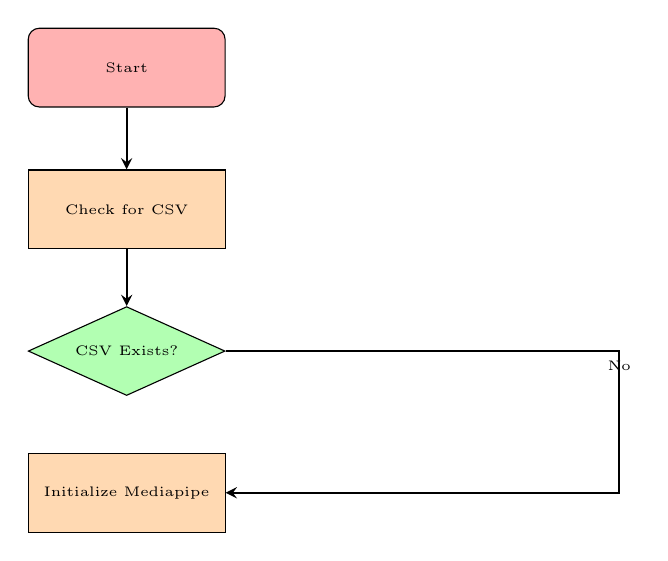
\begin{tikzpicture}[node distance=1.8cm and 2cm, every node/.style={font=\tiny}]
			\node (start) [rectangle, rounded corners, minimum width=2.5cm, minimum height=1cm, text centered, draw=black, fill=red!30] {Start};
			\node (remove_csv) [rectangle, minimum width=2.5cm, minimum height=1cm, text centered, draw=black, fill=orange!30, below of=start] {Check for CSV};
			\node (csv_exists) [diamond, aspect=2, minimum width=2.5cm, minimum height=1cm, text centered, draw=black, fill=green!30, below of=remove_csv] {CSV Exists?};
			\node (init_mediapipe) [rectangle, minimum width=2.5cm, minimum height=1cm, text centered, draw=black, fill=orange!30, below of=csv_exists] {Initialize Mediapipe};
			
			% Arrows
			\draw [thick,->,>=stealth] (start) -- (remove_csv);
			\draw [thick,->,>=stealth] (remove_csv) -- (csv_exists);
			\draw [thick,->,>=stealth] (csv_exists.east) -- ++(5,0) node[anchor=north] {No} |- (init_mediapipe.east);
			%\draw [thick,->,>=stealth] (csv_exists.south) -- ++(0,-1.9) node[anchor=west] {Yes} |- (init_mediapipe.west);
		\end{tikzpicture}
	\end{frame}
	
	% Slide 16: Thank You Slide
	\begin{frame}{Thank You!}
		\centering
		\Huge Thank you for your attention! \\
		\vspace{1cm}
		\large Questions are welcome.
	\end{frame}
	
\end{document}
